%	LaTeX template for the Collaborative Research Center proposal (3rd funding period) Oxyflame.
%	WSA, RWTH Aachen, 2020, (contact person: Stefan Pielsticker)

%%%% PLEASE ADJUST:
%\WorkInstruction{ Enter the number of the project here. Replace only the text "Example project" Please make sure that the project name corresponds exactly to the name of the folder of your project.}
% Example: \renewcommand{\Project}{A1}

\renewcommand{\Project}{A1}
\renewcommand{\ChapterTitle}{Gasphase modelling}
\renewcommand{\ProjectTitle}{Original title from DFG proposal}

\newcommand*\positioncircle[1]{\raisebox{.5pt}{\textcircled{\raisebox{-.9pt} {#1}}}}


%%%% DON'T CHANGE ANYTHING FROM HERE UNTIL NEXT MARKER!
\chapter{\ChapterTitle}
%%%% DONT CHANGE ANYTHING UNTIL HERE!

%%%% PLEASE ADJUST:
\chapterauthor[1]{Anita Meraviglia}
\chapterauthor[1]{Pooria Farmand}
\chapterauthor[2]{Leon Loni Berkel}
\chapterauthor[3]{Stefan Pielsticker}
\chapterauthor[3]{Reinhold Kneer}
\chapterauthor[2]{Christian Hasse}
\chapterauthor[1]{Heinz Pitsch}

%%%% DON'T CHANGE ANYTHING FROM HERE UNTIL NEXT MARKER!
\begin{affils}
	%%%% DONT CHANGE ANYTHING UNTIL HERE!
	
	%%%% PLEASE ADJUST:
	\chapteraffil[1]{\RWTHITV}
	\chapteraffil[2]{\RWTHWSA}
	
%%%% DON'T CHANGE ANYTHING FROM HERE UNTIL NEXT MARKER!
\end{affils}
\begin{refsection}

\begin{abstract}
\label{sec:\Project _Abstract}
%%%% DONT CHANGE ANYTHING UNTIL HERE!

%%%% PLEASE ADJUST
%\WorkInstruction{Title: Keep it short and make sure that it fits well with the part title and the other project titles within that part. Therefore see the planned chapter outline in section~\ref{ex: chap Outline}.}

%\WorkInstruction{Author List: If you use data from FP1/FP2 members, please list them here as well.}

%\WorkInstruction{Affiliations: Please use the commands already prepared (\textbackslash RWTHWSA, \textbackslash RWTHAIA, \textbackslash RWTHITV, \textbackslash RUBLEAT, \textbackslash RUBLTC, \textbackslash RUBThermo, \textbackslash RUBTC, \textbackslash RUBACII, \textbackslash TUDSTFS,\textbackslash TUDRSM, \textbackslash TUDEST. For changes or other affiliations text us.}

\blindtext[2]

\WorkInstruction{Put abstract here, not longer than first page.}

\end{abstract}


\newpage
\section{Introduction} 
Chemical kinetic models are essential when dealing with combustion phenomena as they provide crucial information regarding reaction rates, species transport, and temperature effects. In this Oxyflame project, numerical simulations are performed to analyse the processes in the partially premixed flame resulting from the combustion of solid coal and biomass particles. Like in Cha.~\linkproject{B3}, where solid particle DNS are performed to analyse the combustion and ignition behaviour as well as the main \ce{NO_x} formation pathways, numerical simulations are conducted predominantly under high-temperature air and oxy-fuel conditions at atmospheric pressure in this Oxyflame project. Therefore, with this application in mind, it is necessary to develop a chemical kinetic model to describe the underlying chemistry of the released volatile species in the surrounding gas phase of the solid particle. The latter is determined by employing the solid particle model for coal and biomass devolatilisation from Cha.~\linkproject{A8}, which leads to the definition of a complex mixture ranging from light hydrocarbons and oxygenated species up to heavy lignin tars (\ce{C24H28O4}) and aromatic compounds. Considering the \ce{NO_x} sub-model from Cha.~\linkproject{A8}, various nitrogen-containing species are present, and the introduction in the kinetic model of the relevant chemistry describing their evolution in the combustion system is essential for accounting for the primary \ce{NO_x} formation pathways.
\\
Detailed chemical kinetic models aim to describe the combustion process as accurately as possible. However, this might require hundreds or even thousands of species and reactions. Since the computational cost of complex simulations typically increases as the number of species in the employed kinetic model grows, developing skeletal kinetic models with a reduced number of species and reactions while preserving high accuracy is of key importance for performing the simulation of interest that would be otherwise computationally prohibitive.
\\
Why we need new models and L.Cai ... => focus on oxyconditions and combined with solid model
 

% why we need new chemcial kinetic models: Not only B3 more ...


%\textbf{Chemical kinetic model development}
%\begin{itemize}
%	\item Detailed Chemical kinetic models (ITV-2019 and ITV-2023)
%	\begin{itemize}
%		\item Development of the reduced ITV model (Cai 2020)			% ? one to the top ...
%		\item Development of recent kinetic model
%	\end{itemize}
%	\item Skeletal chemical kinetic model
%	\item Development of \ce{NOx} chemical kinetic submodel
%\end{itemize}
% 
%\textbf{Validation of the kinetic models}
%\begin{itemize}
%	\item Skeletal kinetic model for coal combustion
%	\begin{itemize}
%		\item ITV-2019 (Cai 2020)
%		\item ITV-2023
%	\end{itemize}
%	\item Skeletal kinetic model for biomass combustion
%	\item Validation of \ce{NOx} chemical kinetic submodel
%\end{itemize}
 

\newpage
\section{Chemical kinetic model development}
The development of a chemical kinetic model for coal combustion from Cai et al.~\cite{Cai2020} and recent kinetic models for coal and biomass combustion, as well as a modular \ce{NO_x} sub-model, are presented in this section. Furthermore, the applied methods for developing these chemical kinetic models are described to obtain a compact model size.


\subsection{Development of the reduced ITV-2020 kinetic model}
The final skeletal kinetic model is further reduced to 68 species and 906 reactions model for the application in a DNS.
\\
Different development process ...
 % Liming Cai ????
\\\\
This mechanism was proposed originally by Blanquart et al. (2009) to describe the oxidation of a set of C0-C4 hydrocarbon fuels including methane. In a series of subsequent studies, the mechanism was refined by incorporating the hydrogen mechanism from Burke et al. (2012) and extended to include the reaction schemes of polycyclic aromatic hydrocarbon (PAH) growth (Narayanaswamy et al. 2010) and nitrogen oxide formation (Cai and Pitsch 2015). It has also served as the base chemistry module of a set of chemical mechanisms of biofuel compounds (Cai et al. 2017a, 2019b, c) as well as surrogate components of gasoline and jet fuels (Cai et  al. 2019a; Cai and Pitsch 2015; Narayanaswamy et al. 2016). While this mechanism has been extensively validated for the combustion of fuels in air, it has not yet been validated for experiments using O2/CO2 as oxidizer.



\newpage
\subsection{Development of the skeletal ITV-2023 kinetic models}
The development of recent skeletal kinetic models for coal and biomass combustion involves a multi-step reduction strategy using detailed chemical kinetic models. A schematic of the whole reduction strategy is summarized in Fig.~\ref{fig:B1bKineticModelDevelopmentStructure}.
\\
In the first step, detailed chemical kinetic models have been developed by integrating the chemistry of the missing volatile species from coal and biomass combustion into the model of Langer et al.~\cite{Langer2023}. The model from Langer et al.~\cite{Langer2023} has been systematically extrapolated from recently published chemical kinetic models and combined with recently published detailed chemical kinetic models~\cite{Wagnon2018, Debiagi2016, Pelucchi2015}, describing the missing volatile species chemistry. The so obtained kinetic models are referred to as "Merged-ITV-Cellulose", "Merged-ITV-Propionaldehyde", and "Merged-ITV-Anisole", as shown in Fig.~\ref{fig:B1bKineticModelDevelopmentStructure}. The obtained models undergo a multi-step reduction strategy involving the Direct Relation Graph with Error Propagation (DRGEP) method and Reaction Flux Analysis (RFA). Skeletal kinetic models from each reduction step will be named employing the prefixes "DRGEP-Skeletal" and "RFA-Skeletal", followed by the name of the corresponding detailed chemical kinetic model. The reduction process allows the retention of only the relevant chemistry for the species of interest. This allows the merging process of the skeletal models to be more straightforward, leading to a compact chemical kinetic model (ITV-Compact) able to accurately describe the evolution of the volatile species released from coal and biomass. The obtained compact model is further divided into two skeletal kinetic models via the DRGEP method and the RFA. These skeletal kinetic models describe the gas phase kinetics of volatile species released from coal (Skeletal-ITV-Coal) and biomass (Skeletal-ITV-Bio).
\begin{figure}[h]
  \centering
  \subfloat{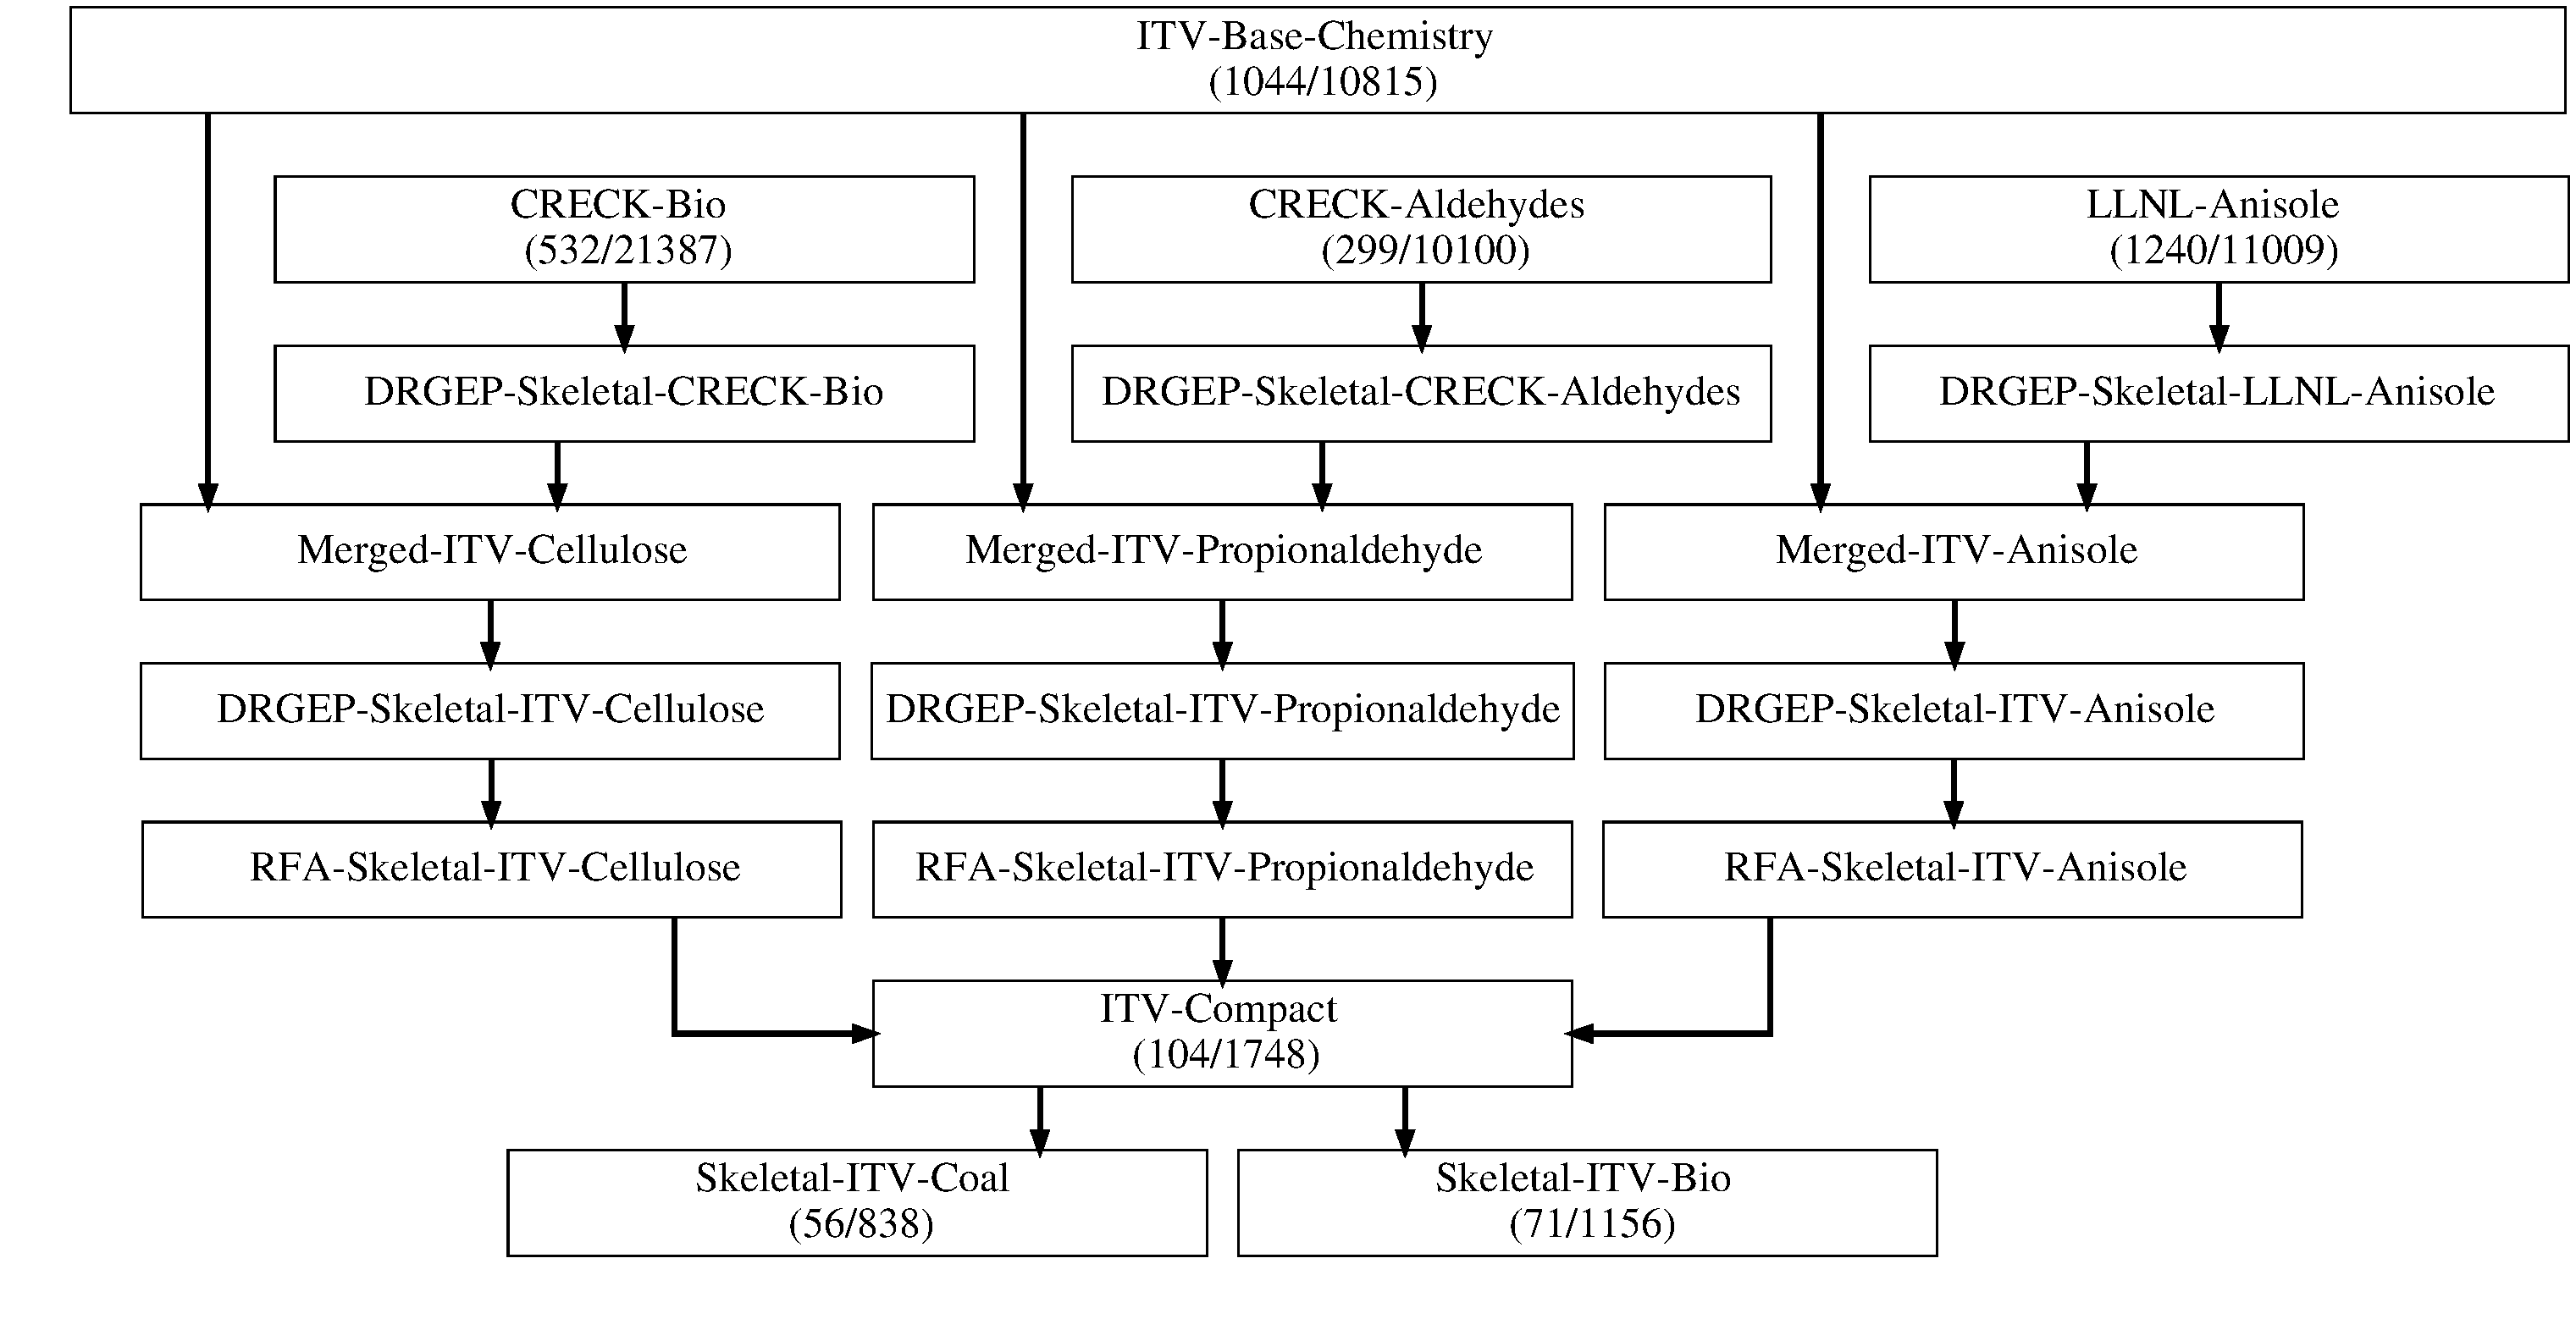
\includegraphics[width=1.0\textwidth]{\ThisPath Figures/B1b_FlowChartMechanismDevelopment.pdf}}
  \caption{Flow chart for developing the skeletal gas phase mechanisms for coal (Skeletal-ITV-Coal) and biomass (Skeletal-ITV-Bio) combustion. The initial mechanisms are the ITV-Base-Chemistry from Langer et al.~\cite{Langer2023}, the LLNL-Anisole~\cite{Wagnon2018}, the CRECK-Bio~\cite{Debiagi2016}, and the CRECK-Aldehydes model~\cite{Pelucchi2015}.}
  \label{fig:B1bKineticModelDevelopmentStructure}
\end{figure}
\\
Further DRGEP reduction steps of these mechanisms using the same validation cases lead to skeletal chemical kinetic mechanisms. A reaction flux analysis allows a flexible and targeted extraction of major formation and consumption pathways of the species of interest from the mechanism. The extraction with the reaction flux analysis was performed based on the respective validation cases to consider the range of validity and application. The extracted models for anisole oxidation, cellulose pyrolysis, and propionaldehyde chemistry are merged into a compact model to obtain a model that can describe all these features.
\\
A compact chemical kinetic model (ITV-Compact) is obtained to capture the prediction for all validation cases for coal and biomass combustion. This model can be used for further mechanism reductions for coal and biomass combustion. The species vanillin and the decomposition reaction for vanillin were added to this compact mechanism from the ITV-Base-Chemistry model~\cite{Langer2023} since it is a major volatile for coal and biomass combustion. Furthermore, isomers of 5-methyl-1,3-cyclopentadiene and the methylcyclopentadienyl radical were lumped based on the approach from Pepiot-Desjardins and Pitsch~\cite{PepiotDesjardins2008b}. The ITV-Compact mechanism contains several volatile species released from the CRECK-S model, which can be used to model coal and biomass combustion and as a basis for further reduction steps.
\\
The final reduction step contains a DRGEP step and an additional reduction step using the reaction flux analysis to obtain skeletal chemical kinetic models for coal and biomass combustion. The applicability of both models can be emphasized by the fact that the Skeletal-ITV-Coal and the Skeletal-ITV-Bio mechanisms contain several volatile species released from the CRECK-S model.
\\
Details about the development steps and the theory of the DRGEP method and the RFA are given below.
 
 
\subsubsection{Detailed chemical kinetic models}
Skeletal kinetic models aim to reproduce combustion characteristics exhibited by detailed models within a specified set of conditions. The latter should be selected to encompass the validity range of the detailed model. From this perspective, having access to a detailed model with strong predictive capabilities across a broad spectrum of experimental conditions constitutes a crucial step in developing a reliable skeletal kinetic model.
\\
In this project, a compact model describing the gas phase kinetics of coal and biomass combustion has been developed by integrating the relevant chemistry of missing volatile species in the extensively validated detailed model from Langer et al.~\cite{Langer2023}. The model from Langer et al.~\cite{Langer2023} is developed to describe the formation of PAH, suitable to describe the soot formation behaviour from biomass combustion. According to the CRECK-S devolatization model described in Cha.~\linkproject{A8}, coal and biomass particles release a complex mixture of volatile species to the gas phase. One of the dominant volatile species released during coal and lignin combustion is anisole, while levoglucosan is the dominant volatile species released from cellulose combustion. To describe the ignition delay time of coal and biomass combustion, the chemistry of anisole and propionaldehyde is considered, the most dominant species released at particle temperatures where biomass ignites is observed, based on model simulations with the solid particle model from Cha. 8. However, these species are not included in the detailed model from Langer et al.~\cite{Langer2023}. To integrate these missing species chemistry in the model from Langer et al.~\cite{Langer2023}, extensively validated detailed chemical kinetic models are used to describe the respective chemistry of interest over a broad range of conditions. The missing anisole chemistry has been adopted from the model of Wagnon et al.~\cite{Wagnon2018}, cellulose volatile species from Debiagi et al.~\cite{Debiagi2016}, and the propionaldehyde chemistry from Pelucchi et al.~\cite{Pelucchi2015}.
\\
The integration of the chemistry, describing the gas-phase kinetics of these volatile species, into the model from Langer et al.~\cite{Langer2023} has been achieved using a systematic approach. In order to extrapolate only the relevant chemistry for the species, the DRGEP method has been applied to these detailed models. The obtained reduced chemical kinetic models are merged into the detailed model from Langer et al.~\cite{Langer2023} based on InChIs and SMILES for each species. Only the species and reactions, as well as the species thermodynamic and transport data, are extracted and added to the chemical kinetic model from Langer et al.~\cite{Langer2023}, which are not included.
\\
The validation database presented in Ref.~\cite{Langer2023} is expanded in this work by integrating additional speciation data representative of anisole oxidation~\cite{Chen2022}, levoglucosan pyrolisis~\cite{Norinaga2013}, and shock tube ignition-delay time measurements of anisole and propionaldehyde~\cite{Pelucchi2015, AkihKumgeh2011}.
% Here add oxyfuel validation (!highlight oxyfuel compability!...)

 

\subsubsection{Skeletal chemical kinetic model}
The skeletal kinetic models for coal and biomass combustion are developed and employed to simulate the gas-phase kinetics of the primary volatile species released during coal and biomass particle combustion under high-temperature and atmospheric pressure conditions. The reduction stage aims to develop chemical kinetic models with a limited number of species while accurately describing the evolution of volatile species under the specific conditions of interest.
\\
However, there is often an opposite trend between the effectiveness of a given kinetic model reduction technique and its computational demand. Based on this, most reduction strategies often consist of faster approaches for reducing detailed chemical kinetic models, where only a species priority list is generated, and numerically more expensive techniques on already reduced models.
\\
Reaction flux-based reduction techniques, such as the DRG~\cite{Lu2005, Lu2020} or DRGEP~\cite{PepiotDesjardins2008a} methods, have the advantage of being very fast in determining a species ranking. These graph-based methods can remove unimportant species from the chemical kinetic model and retain almost all their accuracy. However, increasing the threshold for the reduction leads to an accuracy loss, and the method progressively loses effectiveness. In contrast, a numerically more expensive sensitivity analysis is often applied to reduce skeletal chemical kinetic models. A sensitivity analysis calculates the error on a specific defined target following the removal of each analysed species and ranks them accordingly.
\\
Due to the underlying detailed chemical kinetic models for developing the skeletal models, graph-based reduction techniques are employed to achieve a strongly reduced number of species. Graph-based methodologies allow to schematise the reaction network as a mathematical object, a directed weighted graph which is defined as
\begin{align}
G = \{e,v,w\},
\end{align}
where vertex $v$ represents the species, the edges $e$ connecting two vertexes refer to the reactions, and the weight $w$ defines the strength of the links connecting two species. The definition of the weights varies according to the adopted methodology.


\subsubsection{Directed relation graph with error propagation method}
The directed relation graph with error propagation method~\cite{PepiotDesjardins2008a} is a reliable tool for systematically reducing mechanisms to a skeletal version of itself. The strength of interaction between two directly related species $A$ and $B$ is given with the direct interaction coefficient
\begin{align}
r_{AB} \equiv \frac{|\sum_{j=1}^{N_R} \nu_{j,A}\omega_j\delta_{B}^{j}|}{max(P_A, C_A)},
\end{align}
where the production and consumption rates of target species $A$ are given with
\begin{align}
\label{eq:B1bProductionRate}
P_A = \sum_{j=1}^{N_R} max(0, \nu_{j,A}\omega_j),
\end{align}
\begin{align}
\label{eq:B1bConsumptionRate}
C_A = \sum_{j=1}^{N_R} max(0, -\nu_{j,A}\omega_j).
\end{align}
$N_\mathrm{R}$ is the number of reactions in the kinetic model, $\nu_\mathrm{j}$ is the stoichiometric coefficient, and $\omega_\mathrm{j}$ is the net reaction rate of reaction $j$. $\delta_{B}^{j}$ is unity if the $j$-th reaction involves species $B$ and equals zero otherwise. After calculating the interaction coefficients for all species pairs in the reaction network, a graph search is performed to find all paths from the target species. A path-dependent interaction coefficient on a certain path $p$ that links two species $A$ and $B$, which are not necessarily directly related, represents the error propagation and is defined through a damping procedure as
\begin{align}
r_{AB,p} = \prod_{i=1}^{n-1} r_{S_iS_{i+1}},
\end{align}
where $n$ is the number of species between target species $A$ and species $B$ in pathway $p$ ($S_\mathrm{1}$ = $A$, and $S_\mathrm{n}$ = $B$). The coefficient $R$ represents the introduced error if species $B$ is removed on the prediction of target species $A$ and is defined as the maximum of all path-dependent interaction coefficients between the target species $A$ and each species of interest $B$ of target simulations $T_\mathrm{sim}$:
\begin{align}
R_{AB} \equiv \mathop{max}_{T_{sim}} (\mathop{max}_{\text{all paths } p} (r_{AB,p})).
\end{align}
This target-oriented technique returns a set of species that can be removed from the detailed mechanism with minimal impact on the target species for the range of validity and applicability. The conditions defining the range of validity are both examined counterflow flames from Chen et al.~\cite{Chen2022} measured in the burner from Cha.~\linkproject{B1} for the anisole oxidation chemistry, the secondary pyrolysis of cellulose volatiles species from Norinaga et al.~\cite{Norinaga2013}, and the ignition delay time measurements for propionaldehyde from Pelucchi et al.~\cite{Pelucchi2015} and Akih-Kumgeh and Bergthorson~\cite{AkihKumgeh2011}. The ignition delay time for anisole was validated with anisole/air mixtures at atmospheric pressure. The target species for the DRGEP reduction step were the respective volatile species and additional small \ce{C1} and \ce{C2} hydrocarbons.


\subsubsection{Reaction flux analysis}
Reaction flux analysis generally visualizes the main pathways consuming or producing a certain species. In this mechanism development, the reaction flux analysis tool is employed further to decrease the size of the chemical kinetic model. Unlike the DRGEP method, where the coefficient assigned to a certain species is maximum over all the validation cases, the RFA ensures that the neglected portion of the reaction network is the same over the validation cases.
\\
For a species of interest, a directed graph is created based on the chemical kinetic model to highlight production or consumption pathways, where the vertices are species, and the edges refer to the integrated net reaction flux linking two species. The reaction flux for the production and consumption of a target species $A$ is defined as
\begin{align}
r_{AB} \equiv \frac{|\sum_{j=1}^{N_R} max(0; P_{A,j})\delta_{B}^{j}|}{\sum_{j=1}^{N_R} max(0; P_{A,j})},
\end{align}
\begin{align}
r_{AB} \equiv \frac{|\sum_{j=1}^{N_R} max(0; C_{A,j})\delta_{B}^{j}|}{\sum_{j=1}^{N_R} max(0; C_{A,j})}.
\end{align}
The directed graph is built based on the depth-first-search approach to ensure that every traversed pathway connects target species $A$ with any other species. The direction of the directed graph coincides with the direction of the net reaction rate for consumption or production pathways, respectively. Since all pathways contribute directly or indirectly to the consumption or formation of a target species, a tolerance is defined to consider only the most relevant pathways in the directed graph for the target species $A$. The error propagation approach in the reaction flux analysis is similar to the DRGEP method.
\\
A target species' dominant consumption or production pathways can be extracted from the directed graph based on a simulation that defines the range of applications. However, the remaining fluxes can be neglected from the model without changing the consumption or formation of the target species in the range of validity and applicability. The applied validation simulations defining the range of validity of the skeletal models are the same as those used for the DRGEP method reduction steps. The target species for the reaction flux analysis are the fuel and main pollutants for the ignition delay time extraction, while for the anisole and cellulose chemistry, a more detailed extraction process is applied, considering several small intermediate species as targets with different tolerances.


\subsection{Development of a \ce{NOx} chemical kinetic submodel}
To describe the formation of \ce{NO_x} from nitrogen-containing volatile species released from the CRECK-S model, a chemical kinetic gas-phase model for \ce{NO_x} formation is newly developed. This newly developed chemical kinetic model uses an ITV-\ce{NO_x} model, a reduced version of the well-documented Glarborg et al. model~\cite{Glarborg2018}, crafted through ab-initio and experimental studies, as base chemistry. Based on a quantitative assessment of ammonia and ammonia/hydrogen combustion of different chemical kinetic models, Girhe et al.~\cite{Girhe2024} reported satisfactory results under most of the examined experimental conditions for the KAUST ammonia model~\cite{Zhang2021}. Based on this study, the ITV integrates the ammonia chemistry from the KAUST model to the reduced Glaborg model to improve the predictions of the ammonia chemistry. The required pyridine chemistry to model tar-N is adopted from the CRECK-\ce{NO_x} model~\cite{Shamooni2021} and integrated into the base-chemistry model from the ITV.
\\
However, this merged ITV-\ce{NO_x} model over-predicts the \ce{NO} formation over a broad range of experimental conditions. Comparing the \ce{NO} formation pathways from the ITV-\ce{NO_x} model and the CRECK-\ce{NO_x} model~\cite{Shamooni2021}, which is able to capture the \ce{NO} formation accurately, reveals an over-predicted \ce{NCO}-chemistry in the ITV-\ce{NO_x} model. The dominant \ce{NO} formation reactions via the \ce{NCO} radical differ in both kinetic models, while the most dominant \ce{NCO} consumption reaction in the ITV-\ce{NO_x} model is
\begin{align}
\ce{NCO}+\ce{O} \Leftrightarrow \ce{NO}+\ce{CO}.
\end{align}
To slow down this \ce{NO} formation pathway, the tuned reaction rate from the CRECK-\ce{NO_x} model~\cite{Shamooni2021} is adopted to the ITV-\ce{NO_x} model. With this reaction rate modification, the \ce{NCO} pathway is slowed down and the \ce{NH}-chemistry becomes more important for the \ce{NO} formation, resulting in an accurately predicted NO formation. However, this modification results in an over-predicted \ce{N2O}-chemistry. A slightly reduced frequency parameter for the most dominant \ce{N2O} formation reaction in the ITV-\ce{NO_x} model
\begin{align}
\ce{NCO}+\ce{NO} \Leftrightarrow \ce{N2O}+\ce{CO},
\end{align}
slows down this \ce{N2O} formation pathway and results in an accurate \ce{N2O} prediction.
\\
Next to the rate modifications, the nitrogen chemistry in the Complete-ITV-\ce{NO_x} model is extracted using the reaction flux analysis to obtain a more compact model size. The target species for the extraction are the volatile species released from the solid particle models. Using a very tiny tolerance for the flux analysis and considering the validation cases from Alzueta et al.~\cite{Alzueta2002} and Wu et al.~\cite{Wu2019, Wu2022}, an extracted kinetic model is obtained, which covers a broad spectrum of fuel-air ratios, temperatures, and initial conditions. The Skeletal-ITV-\ce{NO_x} is a generally applicable modular chemical kinetic model for \ce{NO_x} formation containing 36 species and 595 reactions.
% R1 not Eq????




\newpage
\section{Validation of kinetic models}
The ITV-2023 skeletal chemical kinetic models for coal and biomass are developed to predict the ignition delay time and respective fuel chemistry based on detailed chemical kinetic models. However, due to the reduction of detailed chemical kinetic models, the prediction accuracy of the chemistry of several species is affected. Consequently, a comprehensive validation is required to cover all relevant fuels and target species and include ignition delay times and speciation data in a broad range of temperatures at atmospheric pressure. Numerical simulations for the validation are performed using appropriate models in the FlameMaster code~\cite{Pitsch1990}.

% TODO: The ITV-2020 model~\cite{Cai2020} for coal combustion

 
\subsection{Skeletal kinetic models for coal combustion}
This subsection provides a brief overview of the validation of the ITV-2020 model~\cite{Cai2020} and a more detailed validation of the ITV-2023 kinetic model for coal combustion.


\subsubsection{ITV-2020}
Figure~\ref{fig:B1bIDTLimingCaiCoalMechanism} shows model predictions of the ITV-2020 model~\cite{Cai2020} in comparison with experimental shock-tube measurements from Koroglu et al.~\cite{Koroglu2016}. Koroglu et al.~\cite{Koroglu2016} uses \ce{CH4}/\ce{O2}/\ce{CO2} mixtures in bath gas of \ce{Ar} to measure the ignition delay time for different pressures in the range of \SI{0.61}{atm} to \SI{3.92}{atm} and equivalence ratios of 0.5, 1.0, and 2.0 for \ce{CO2} mole fractions of \SI{30}{\%} and \SI{60}{\%}. The ITV-2020 model~\cite{Cai2020} satisfactorily predicts the ignition delay times for all conditions and temperature ranges.
\\
Further validation cases for oxy-methane combustion can be found in Ref.~\cite{Cai2020}.
% Ignition delay time validation - Koroglu
\begin{figure}[h]
  \centering
  \subfloat{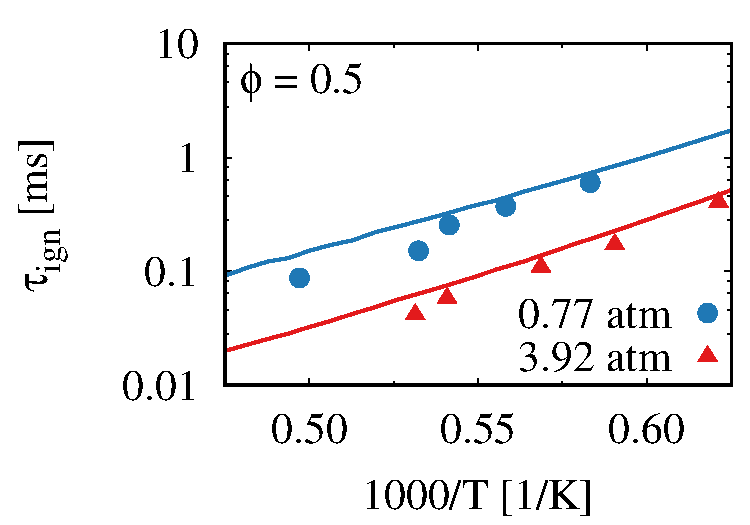
\includegraphics[width=0.48\textwidth]{\ThisPath Figures/B1b_LCai_IDT_CH4_Koroglu_Lean.pdf}}
  \hfill
  \subfloat{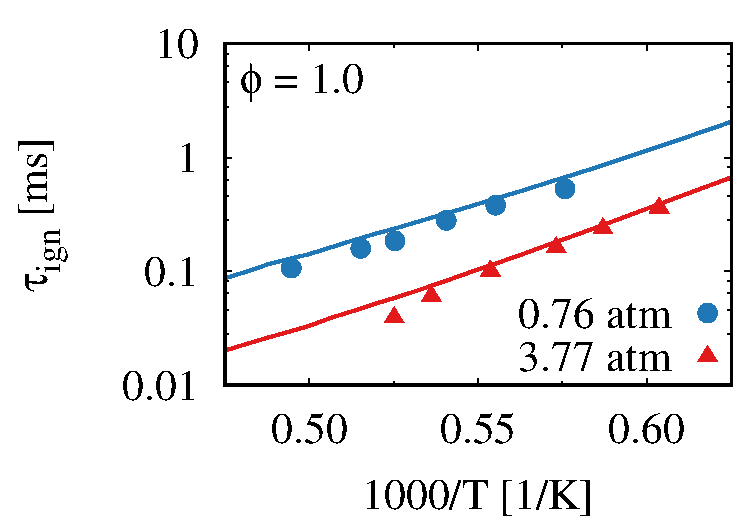
\includegraphics[width=0.48\textwidth]{\ThisPath Figures/B1b_LCai_IDT_CH4_Koroglu_Stoi.pdf}}
  \hfill
  \subfloat{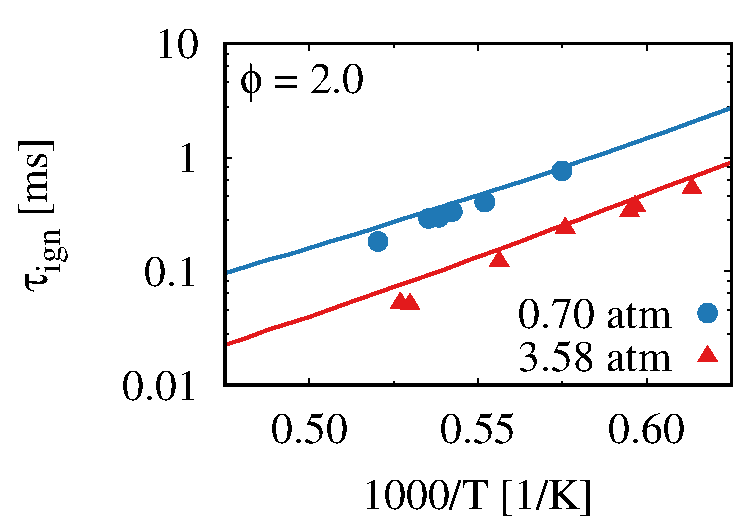
\includegraphics[width=0.48\textwidth]{\ThisPath Figures/B1b_LCai_IDT_CH4_Koroglu_Rich.pdf}}
  \hfill
  \subfloat{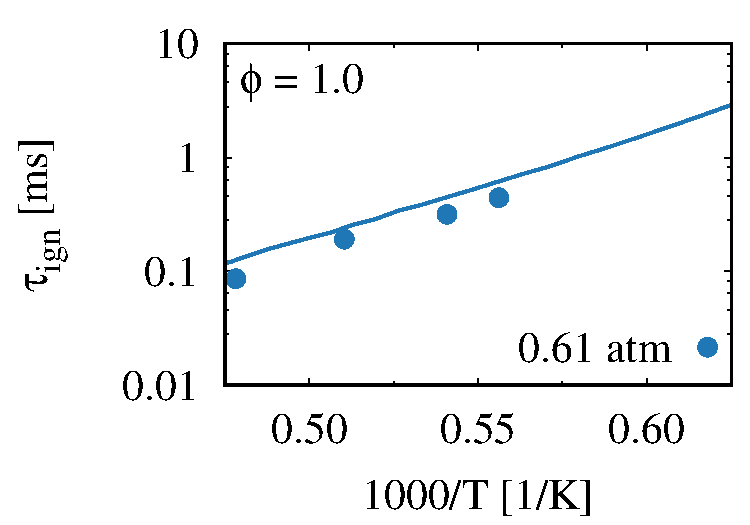
\includegraphics[width=0.48\textwidth]{\ThisPath Figures/B1b_LCai_IDT_CH4_Koroglu_Stoi_XCO2_060.pdf}}
  \caption{Comparison of experimental measured ignition delay times of \ce{CH4}/\ce{O2}/\ce{CO2}/\ce{Ar} mixtures from Koroglu et al.~\cite{Koroglu2016} and model prediction of the ITV-2020 model~\cite{Cai2020}.}
  \label{fig:B1bIDTLimingCaiCoalMechanism}
\end{figure}



\subsubsection{ITV-2023}
The coal skeletal model is validated by considering the oxidation of anisole at atmospheric pressure over a broad range of temperatures. Quantities predicted by the skeletal model are compared against the ones of the corresponding detailed model to assess the effect induced by the reduction phase. Additionally, to assess the influence of differing base chemistry, the performance of the ITV-based detailed chemical kinetic model is evaluated against both the reference models and, where possible, experimental data. The skeletal chemical kinetic model for coal combustion is validated against the measured data for anisole oxidation from Chen et al.~\cite{Chen2022} in two counterflow diffusion flames at atmospheric pressure. Since experimental data for the ignition delay time of anisole at atmospheric pressure are not present in the literature, the ignition delay time of anisole is compared to the model predictions of the respective detailed chemical kinetic models. The detailed chemical kinetic model from Wagnon et al.~\cite{Wagnon2018} and the Merged-ITV-Anisole mechanism serve as a reference for the skeletal chemical kinetic model in both cases.
\\\\
The ignition delay time for anisole is validated for three different fuel-air-equivalence ratios over a broad range of temperatures. Figure~\ref{fig:B1bIDTAnisoleCoalMechanism} compares the prediction for the ignition delay time of anisole/air mixtures for the Skeletal-ITV-Coal, the Merged-ITV-Anisole, and the LLNL-Anisole model~\cite{Wagnon2018} chemical kinetic model. The model from Wagnon et al.~\cite{Wagnon2018} predicts a longer ignition delay time for the examined temperature range for all three fuel-air-equivalence ratios than the Merged-ITV-Anisole and the Skeletal-ITV-Coal model. Predictions for the ignition delay times of the Skeletal-ITV-Coal and the Merged-ITV-Anisole model are similar, indicating a low error in the mechanism reduction process. Deviations to the reference LLNL-Anisole model~\cite{Wagnon2018} are constant for all conditions, while for the fuel-rich case, a slightly higher deviation is predicted. The difference in the prediction of the ignition delay time compared to the LLNL-Anisole model~\cite{Wagnon2018} is based on the different base chemistry in the models.
% Ignition delay time validation
\begin{figure}[h]
  \centering
  \subfloat{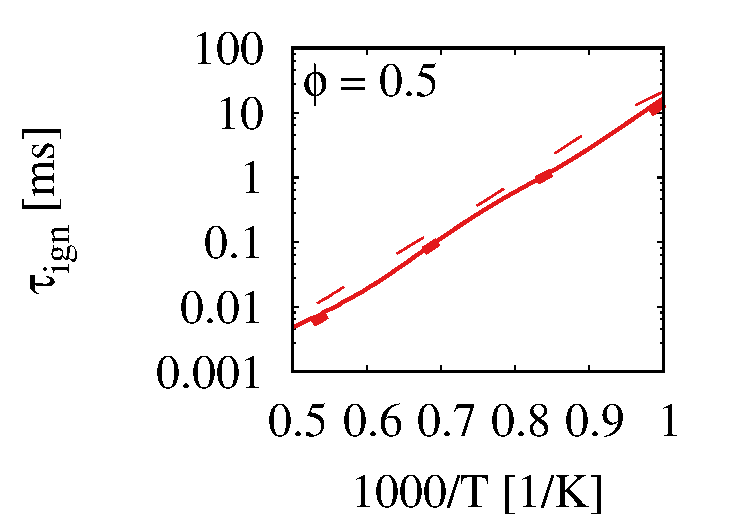
\includegraphics[width=0.32\textwidth]{\ThisPath Figures/B1b_Coal_IDT_Lean_1atm.pdf}}
  \hfill
  \subfloat{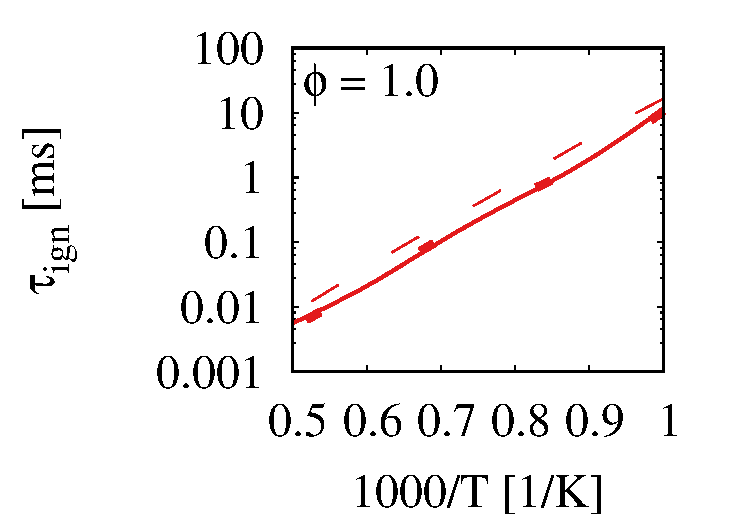
\includegraphics[width=0.32\textwidth]{\ThisPath Figures/B1b_Coal_IDT_Stoichiometric_1atm.pdf}}
  \hfill
  \subfloat{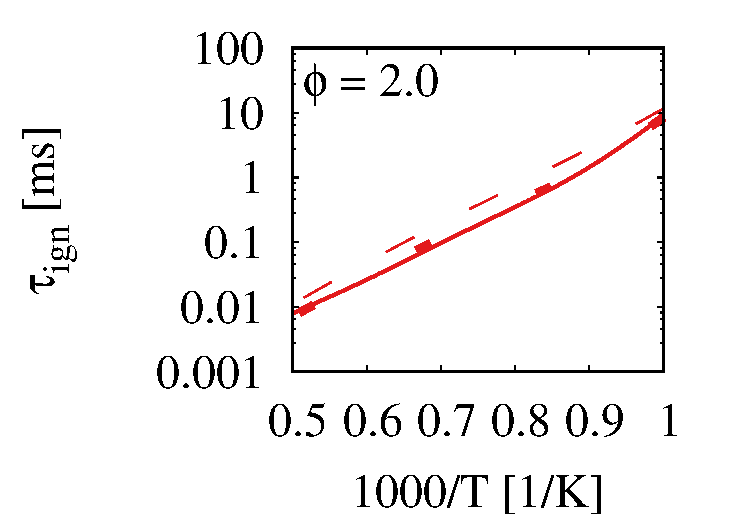
\includegraphics[width=0.32\textwidth]{\ThisPath Figures/B1b_Coal_IDT_Rich_1atm.pdf}}
  \caption{Model comparison for the ignition delay times of anisole/air mixtures at atmospheric pressure for the Skeletal-ITV-Coal model (solid lines), the Merged-ITV-Anisole model (dotted lines), and the LLNL-Anisole model~\cite{Wagnon2018} (dashed lines).}
  \label{fig:B1bIDTAnisoleCoalMechanism}
\end{figure}
\\
%Anisole is one of the most dominant volatile species released during coal combustion.
Validation of the anisole oxidation chemistry for the Skeletal-ITV-Coal model is given based on both examined flame configurations from Chen et al.~\cite{Chen2022}. The examined flame configurations from Chen et al.~\cite{Chen2022} contain carbon dioxide as diluent on the fuel-side (\ce{CO2}F-Flame) or on the oxidizer side (\ce{CO2}O-Flame) to represent oxy-fuel conditions as discussed in Cha.~\linkproject{B1}. Figure~\ref{fig:B1bAnisoleOxidationCoalMechanismCO2F} and~\ref{fig:B1bAnisoleOxidationCoalMechanismCO2O} compare the Skeletal-ITV-Coal model with the respective detailed kinetic model predictions in both counterflow flame configurations from Chen et al.~\cite{Chen2022}. Anisole and the main pollutants \ce{CO} and \ce{CO2} model predictions of the Skeletal-ITV-Coal model show no discrepancies to the detailed LLNL-Anisole~\cite{Wagnon2018} and the Merged-ITV-Anisole for both flame configurations. Only the peak mole fraction of \ce{CO} is slightly over-predicted with the Skeletal-ITV-Coal model compared to the detailed chemical kinetic models, resulting from the mechanism reduction process. Model predictions of the Skeletal-ITV-Coal model for intermediate hydrocarbons like \ce{C2H2} and \ce{A-C3H4} capture the GC-MS measured mole fraction peak for both flame configurations, while the Merged-ITV-Coal and the LLNL-Anisole model~\cite{Wagnon2018} are both under-predicting the mole fraction peak. Missing formation pathways in the Skeletal-ITV-Coal model introduce an error in the formation of this species, which results in an accurate prediction due to the mechanism reduction procedure. Like intermediate species, the Skeletal-ITV-Coal model can capture the mole fraction peak of aromatic species like \ce{A1OH} with a compact model size similar to the detailed chemical kinetic models as shown in Fig.~\ref{fig:B1bAnisoleOxidationCoalMechanismCO2F} and~\ref{fig:B1bAnisoleOxidationCoalMechanismCO2O}.
% Ansiole oxidation chemistry
\begin{figure}[h]
  \centering
  \subfloat{\includegraphics[width=0.32\textwidth]{\ThisPath Figures/B1b_Coal_Figure_3a.pdf}}
  \hfill
  \subfloat{\includegraphics[width=0.32\textwidth]{\ThisPath Figures/B1b_Coal_Figure_3e.pdf}}
  \hfill
  \subfloat{\includegraphics[width=0.32\textwidth]{\ThisPath Figures/B1b_Coal_Figure_3f.pdf}}
  \hfill
  \subfloat{\includegraphics[width=0.32\textwidth]{\ThisPath Figures/B1b_Coal_Figure_7b.pdf}}
  \hfill
  \subfloat{\includegraphics[width=0.32\textwidth]{\ThisPath Figures/B1b_Coal_Figure_7h.pdf}}
  \hfill
  \subfloat{\includegraphics[width=0.32\textwidth]{\ThisPath Figures/B1b_Coal_Figure_12a.pdf}}
  \caption{Comparison of experimentally measured mole fractions in the \ce{CO2}F-Flame for anisole oxidation from Chen et al.~\cite{Chen2022} using the ToF-MBMS (red crosses), the GC-MS with a Rt-Q-Bond column (green circles), and the GC-MS with a DB-Petro column (blue triangles) with model predictions of the Skeletal-ITV-Coal (solid lines), the Merged-ITV-Anisole (dotted lines), and the LLNL-Anisole model~\cite{Wagnon2018} (dashed lines). Shaded areas with different colors indicate the measurement uncertainty of the respective techniques. x refers to the distance from the fuel inlet at 0 mm to the oxidizer inlet at 10 mm.}
  \label{fig:B1bAnisoleOxidationCoalMechanismCO2F}
\end{figure}
\begin{figure}[h]
  \centering
  \subfloat{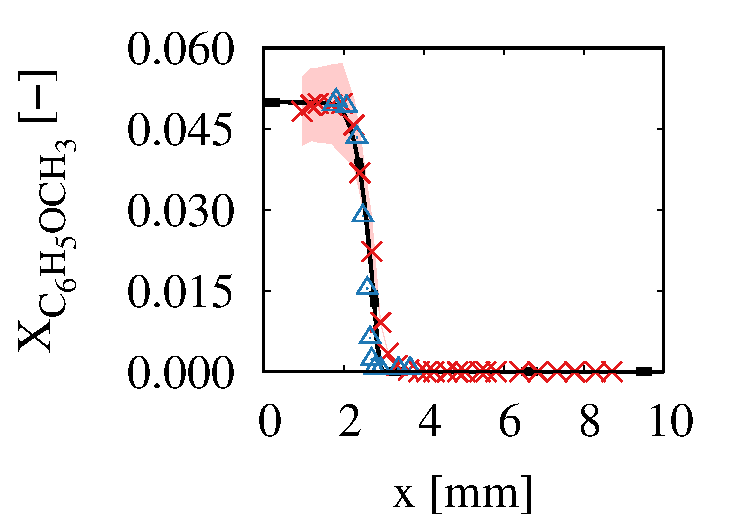
\includegraphics[width=0.32\textwidth]{\ThisPath Figures/B1b_Coal_Figure_6a.pdf}}
  \hfill
  \subfloat{\includegraphics[width=0.32\textwidth]{\ThisPath Figures/B1b_Coal_Figure_6e.pdf}}
  \hfill
  \subfloat{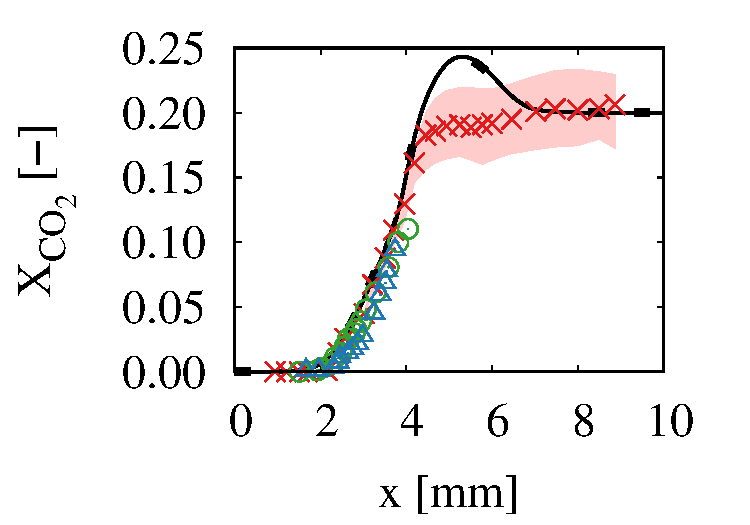
\includegraphics[width=0.32\textwidth]{\ThisPath Figures/B1b_Coal_Figure_6f.pdf}}
  \hfill
  \subfloat{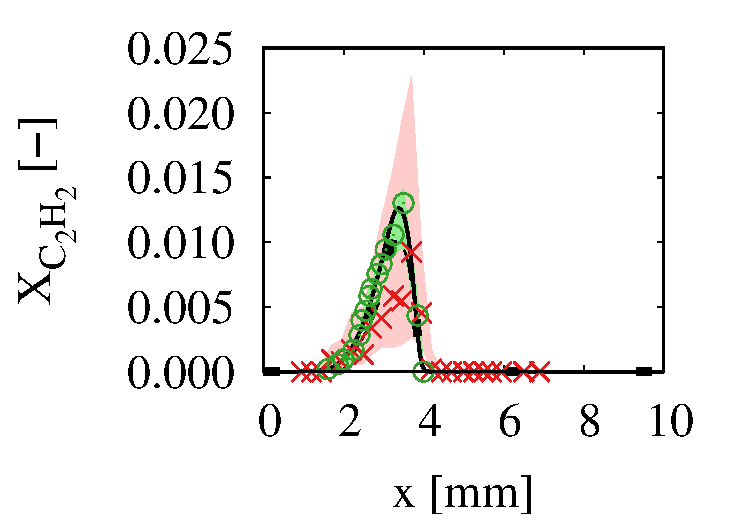
\includegraphics[width=0.32\textwidth]{\ThisPath Figures/B1b_Coal_Figure_8b.pdf}}
  \hfill
  \subfloat{\includegraphics[width=0.32\textwidth]{\ThisPath Figures/B1b_Coal_Figure_8h.pdf}}
  \hfill
  \subfloat{\includegraphics[width=0.32\textwidth]{\ThisPath Figures/B1b_Coal_Figure_13a.pdf}}
  \caption{Comparison of experimentally measured mole fractions in the \ce{CO2}O-Flame for anisole oxidation from Chen et al.~\cite{Chen2022} using the ToF-MBMS (red crosses), the GC-MS with a Rt-Q-Bond column (green circles), and the GC-MS with a DB-Petro column (blue triangles) with model predictions of the Skeletal-ITV-Coal (solid lines), the Merged-ITV-Anisole (dotted lines), and the LLNL-Anisole model~\cite{Wagnon2018} (dashed lines). Shaded areas with different colors indicate the measurement uncertainty of the respective techniques. x refers to the distance from the fuel inlet at 0 mm to the oxidizer inlet at 10 mm.}
  \label{fig:B1bAnisoleOxidationCoalMechanismCO2O}
\end{figure}



\subsection{Skeletal kinetic model for biomass combustion}
 Applying the newly developed skeletal kinetic model for biomass combustion in a DNS requires a detailed validation of the ignition delay time and the chemistry of levoglucosan and anisole in a predefined range of validity. The Skeletal-ITV-Bio model is built on the detailed chemical kinetic models of CRECK-Aldehydes~\cite{Pelucchi2015}, CRECK-Bio~\cite{Debiagi2016}, LLNL-Anisole~\cite{Wagnon2018}, and the updated ITV-Base-Chemistry~\cite{Langer2023}. These detailed chemical kinetic models are validated against data from several experimental species over various conditions. The newly developed Skeletal-ITV-Bio kinetic model will be validated for the ignition delay time of propionaldehyde, secondary pyrolysis of cellulose volatile species, and for the anisole oxidation chemistry against experimental data~\cite{Pelucchi2015, AkihKumgeh2011, Norinaga2013, Chen2022}.
\\\\
The ignition delay time for propionaldehyde is validated for three different fuel-air-equivalence ratios over a broad range of temperatures with experimental shock-tube measurements from Pelucchi et al.~\cite{Pelucchi2015} and Akih-Kumgeh and Bergthorson~\cite{AkihKumgeh2011}. Figure~\ref{fig:B1bIDTPropionaldehydeBioMechanism} compares the model prediction of the Skeletal-ITV-Bio model with the model predictions of the Merged-ITV-Propanal and the CRECK-Aldehydes model~\cite{Pelucchi2015} and with experimental measurements~\cite{Pelucchi2015, AkihKumgeh2011}. Experimental shock-tube measurements are accurately predicted for both examined validation cases with all chemical kinetic models. The detailed chemical kinetic CRECK-Aldehydes model~\cite{Pelucchi2015} predicts a shorter ignition delay time as the Merged-ITV-Propanal and Skeletal-ITV-Bio model for all examined conditions in Fig.~\ref{fig:B1bIDTPropionaldehydeBioMechanism} due to the different base chemistry. No significant discrepancies are shown between the Skeletal-ITV-Bio and the Merged-ITV-Bio for all validation cases, indicating that the mechanism development process introduced only a minor uncertainty in the ignition delay time prediction.
% Ignition delay time validation
\begin{figure}[h]
  \centering
  \subfloat{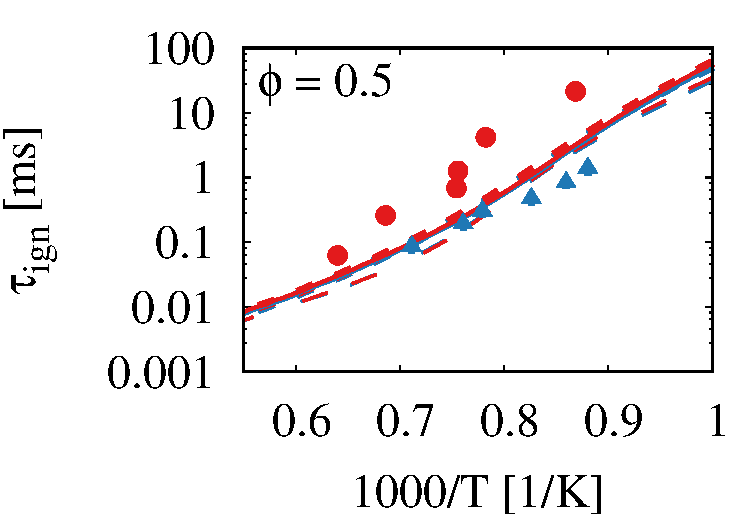
\includegraphics[width=0.32\textwidth]{\ThisPath Figures/B1b_Bio_IDT_Propanal_Lean.pdf}}
  \hfill
  \subfloat{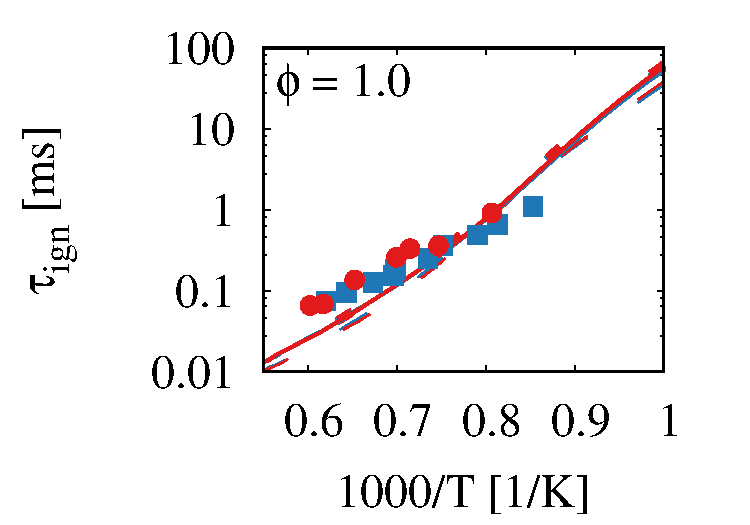
\includegraphics[width=0.32\textwidth]{\ThisPath Figures/B1b_Bio_IDT_Propanal_Stoichiometric.pdf}}
  \hfill
  \subfloat{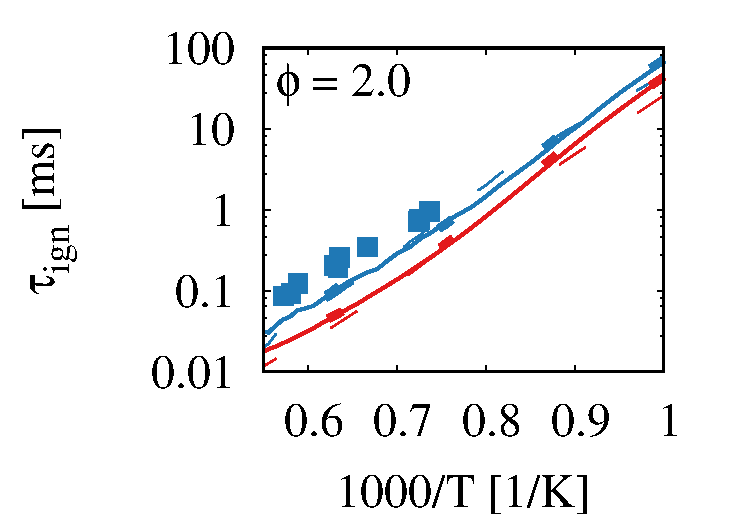
\includegraphics[width=0.32\textwidth]{\ThisPath Figures/B1b_Bio_IDT_Propanal_Rich.pdf}}
  \caption{Comparison of the propionaldehyde ignition delay time for experimental shock-tube measurements from Pelucchi et al.~\cite{Pelucchi2015} (blue squares) and from Akih-Kumgeh and Bergthorson~\cite{AkihKumgeh2011} (black circles) with model predictions of the Skeletal-ITV-Bio model (solid lines), the Merged-ITV-Anisole model (dotted lines), and the CRECK-Aldehydes model~\cite{Pelucchi2015} (dashed lines).}
  \label{fig:B1bIDTPropionaldehydeBioMechanism}
\end{figure}
\\
Experimental measurements in a tubular flow reactor by Norinaga et al.~\cite{Norinaga2013} are used as validation cases for the mechanism development procedure for the secondary pyrolysis of volatile cellulose components like levoglucosan. Some species in the initial composition of the experiment are not considered target species during the development procedure and are removed from the model to achieve a skeletal model size. Therefore, validating the experimental data with the newly developed Skeletal-ITV-Bio model is not meaningful. A purely model validation for the secondary pyrolysis of volatile species is shown in Fig.~\ref{fig:B1bCellulosePyrolysisBioMechanism}. The initial conditions are based on the experiment from Norinaga et al.~\cite{Norinaga2013} using levoglucosan as a balance for all species not included in the Skeletal-ITV-Bio model. Model predictions for levoglucosan, the main pollutants \ce{CO} and \ce{CO2}, intermediate species (\ce{C2H4} and \ce{C2H5CHO}), and aromatic species (\ce{A1}) for the Skeletal-ITV-Bio and the Merged-ITV-Cellulose show no discrepancies. The discrepancies shown for \ce{CO2} and \ce{A1} between the Merged-ITV-Cellulose and the CRECK-Bio model~\cite{Debiagi2016} at higher temperature result from a different underlying base chemistry.
% Cellulose pyrolysis validation
\begin{figure}[h]
  \centering
  \subfloat{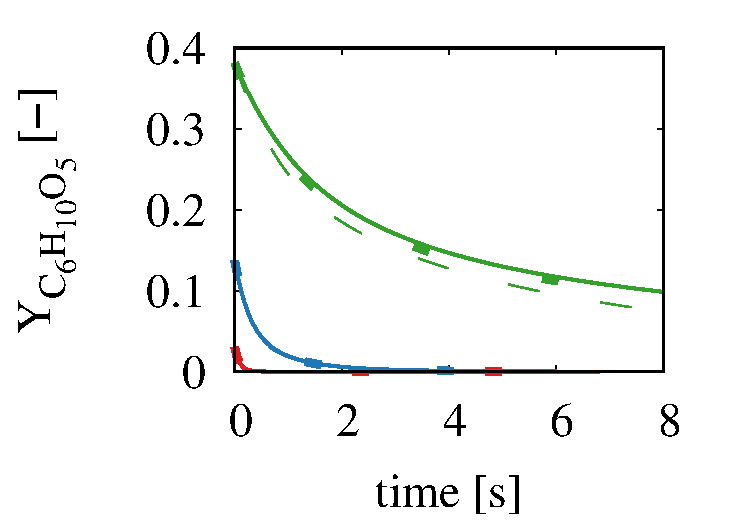
\includegraphics[width=0.32\textwidth]{\ThisPath Figures/B1b_Bio_CellulosePyrolysis_C6H10O5.pdf}}
  \hfill
  \subfloat{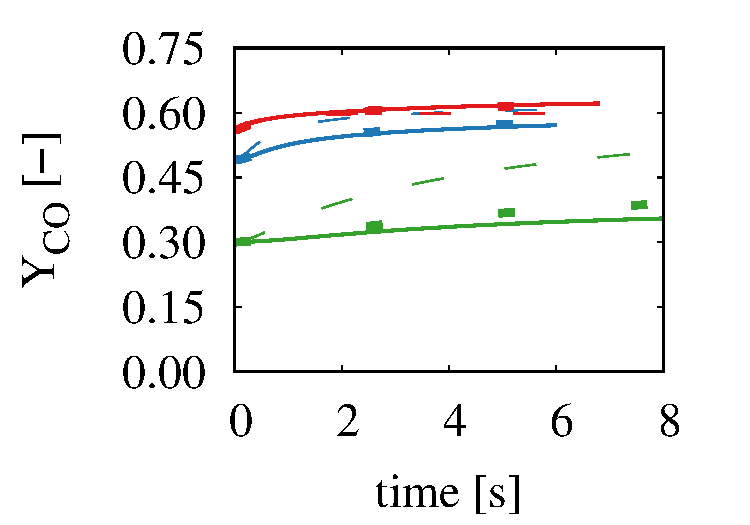
\includegraphics[width=0.32\textwidth]{\ThisPath Figures/B1b_Bio_CellulosePyrolysis_CO.pdf}}
  \hfill
  \subfloat{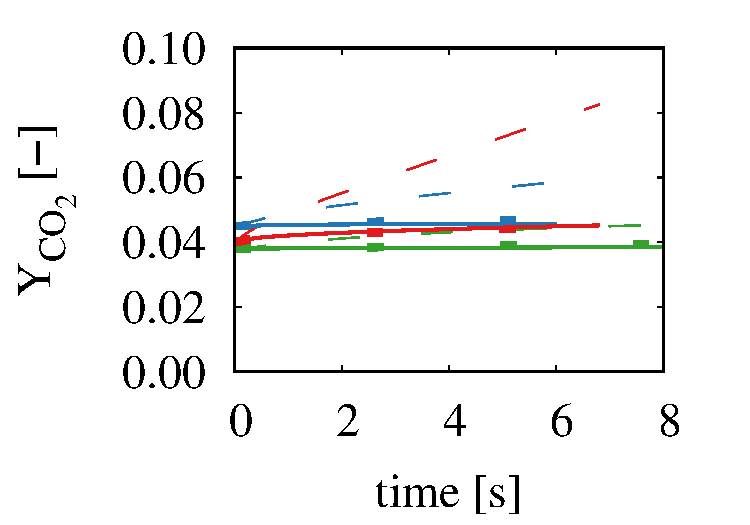
\includegraphics[width=0.32\textwidth]{\ThisPath Figures/B1b_Bio_CellulosePyrolysis_CO2.pdf}}
  \hfill
  \subfloat{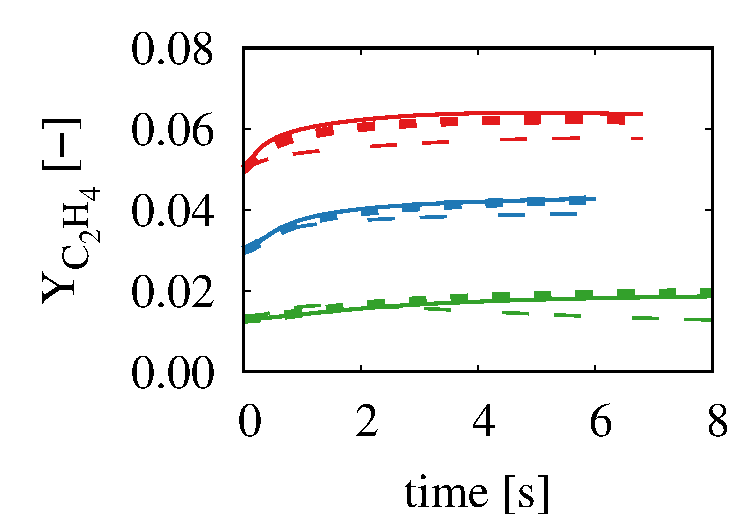
\includegraphics[width=0.32\textwidth]{\ThisPath Figures/B1b_Bio_CellulosePyrolysis_C2H4.pdf}}
  \hfill
  \subfloat{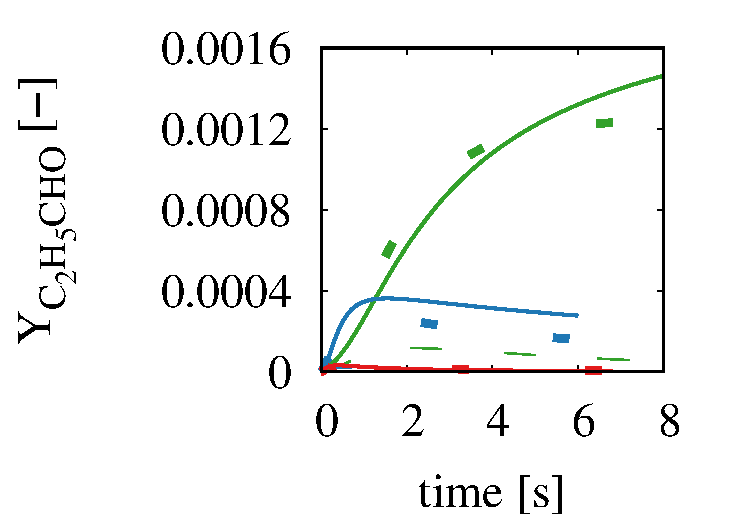
\includegraphics[width=0.32\textwidth]{\ThisPath Figures/B1b_Bio_CellulosePyrolysis_C2H5CHO.pdf}}
  \hfill
  \subfloat{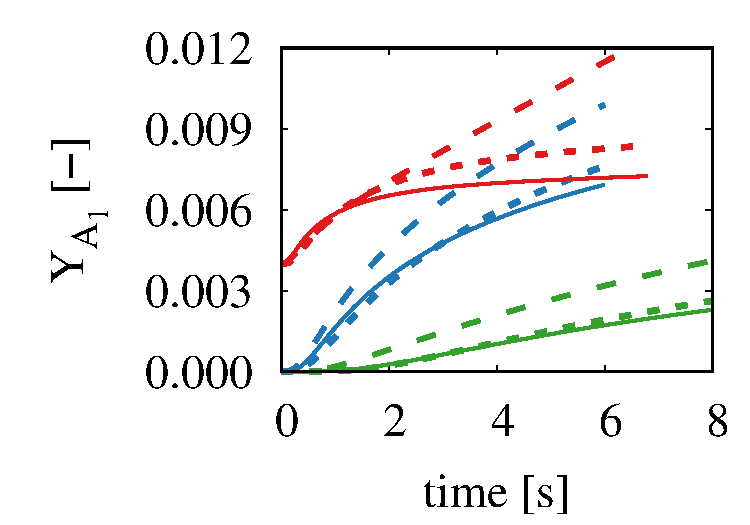
\includegraphics[width=0.32\textwidth]{\ThisPath Figures/B1b_Bio_CellulosePyrolysis_C6H6.pdf}}
  \caption{Model comparison for the secondary pyrolysis of cellulose volatile species at \SI{700}{\celsius} (green), \SI{750}{\celsius} (blue), and \SI{800}{\celsius} (red) for the SkeletalITV-Bio (solid lines), the Merged-ITV-Cellulose (dotted lines), and the CRECK-Bio model~\cite{Debiagi2016}.}
  \label{fig:B1bCellulosePyrolysisBioMechanism}
\end{figure}
\\
A validation of the lignin part of the Skeletal-ITV-Bio model is required to cover all aspects of the Skeletal-ITV-Bio model. The main volatile species released during lignin combustion is anisole. The validation cases for anisole oxidation are both counterflow flame configurations from Chen et al.~\cite{Chen2022} similar to the Skeletal-ITV-Coal model validation. Anisole and the main pollutants \ce{CO} and \ce{CO2} are well predicted for the Skeletal-ITV-Bio model in comparison to the Merged-ITV-Anisole and the LLNL-Anisole model~\cite{Wagnon2018} as shown in Fig.~\ref{fig:B1bAnisoleOxidationBioMechanism} and ~\ref{fig:B1bAnisoleOxidationBioMechanismOXY}. Due to an introduced error from the multi-step reduction procedure, the Skeletal-ITV-Bio model can capture the mole fraction peak of \ce{C5H6}, while the respective detailed kinetic models under-predict the experimentally measured mole fraction peak. However, despite these advantages of more accurate predictions than the detailed reference model, some significant discrepancies exist between the ITV-Skeletal-Bio and the Merged-ITV-Anisole model. These discrepancies result from missing species and pathways in the Skeletal-ITV-Bio model, which are neglected in the development phase due to the requirement of a compact model size. An over-predicted mole fraction peak can be seen for \ce{A1OH} and \ce{C2H2} in Fig.~\ref{fig:B1bAnisoleOxidationBioMechanism} and~\ref{fig:B1bAnisoleOxidationBioMechanismOXY}.
 % Anisole oxidation chemistry validation
\begin{figure}[h]
  \centering
  \subfloat{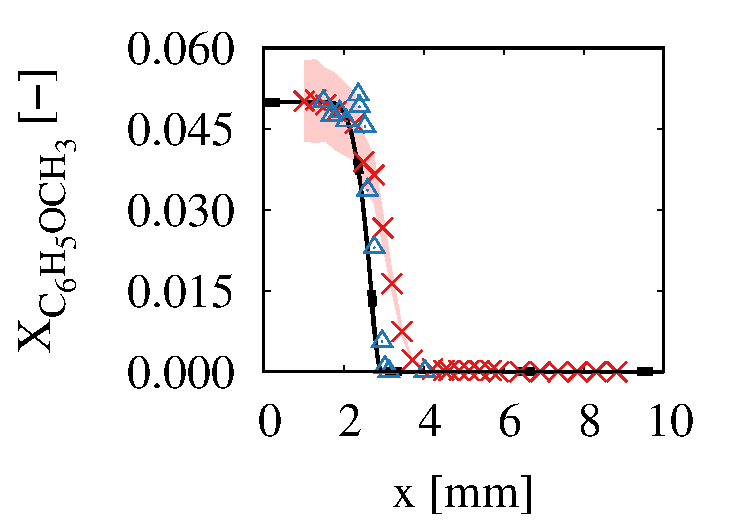
\includegraphics[width=0.32\textwidth]{\ThisPath Figures/B1b_Bio_Figure_3a.pdf}}
  \hfill
  \subfloat{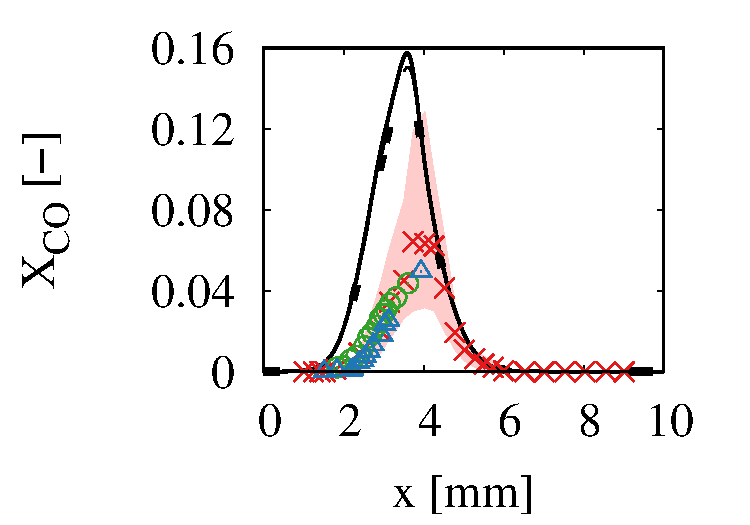
\includegraphics[width=0.32\textwidth]{\ThisPath Figures/B1b_Bio_Figure_3e.pdf}}
  \hfill
  \subfloat{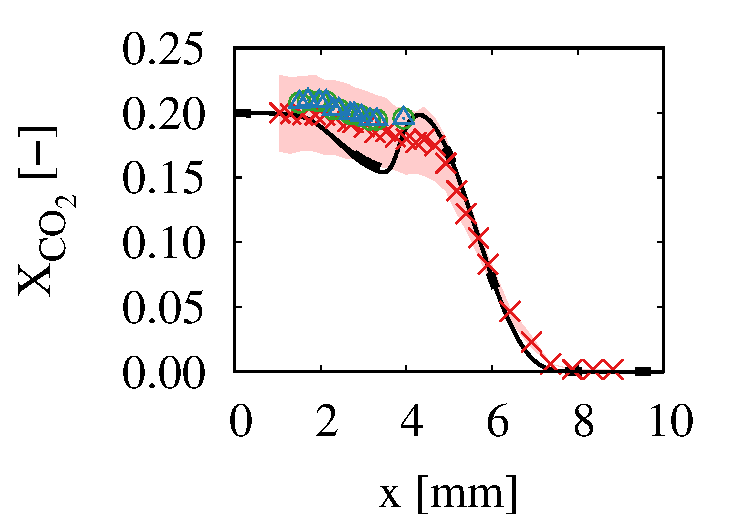
\includegraphics[width=0.32\textwidth]{\ThisPath Figures/B1b_Bio_Figure_3f.pdf}}
  \hfill
  \subfloat{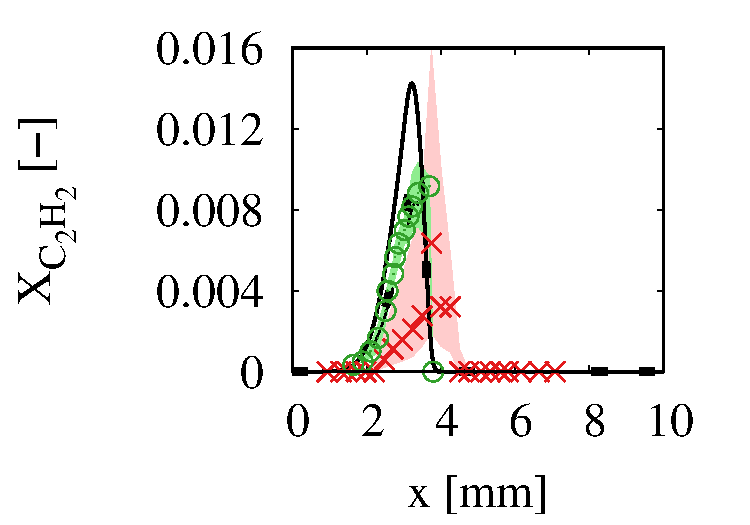
\includegraphics[width=0.32\textwidth]{\ThisPath Figures/B1b_Bio_Figure_7b.pdf}}
  \hfill
  \subfloat{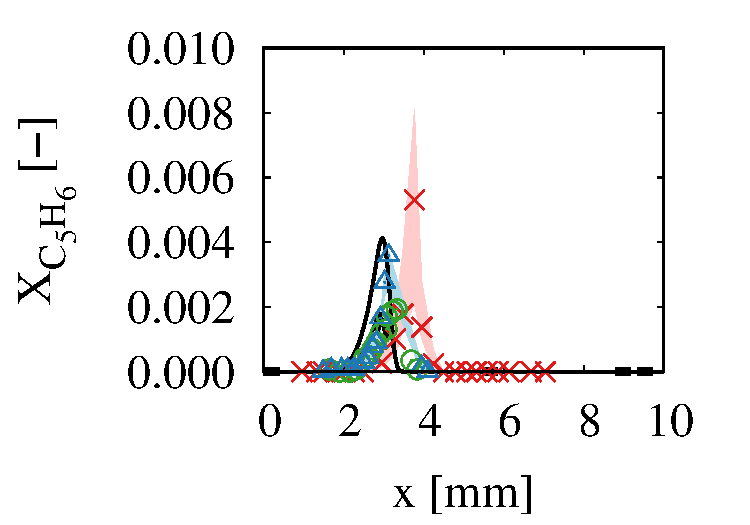
\includegraphics[width=0.32\textwidth]{\ThisPath Figures/B1b_Bio_Figure_7e.pdf}}
  \hfill
  \subfloat{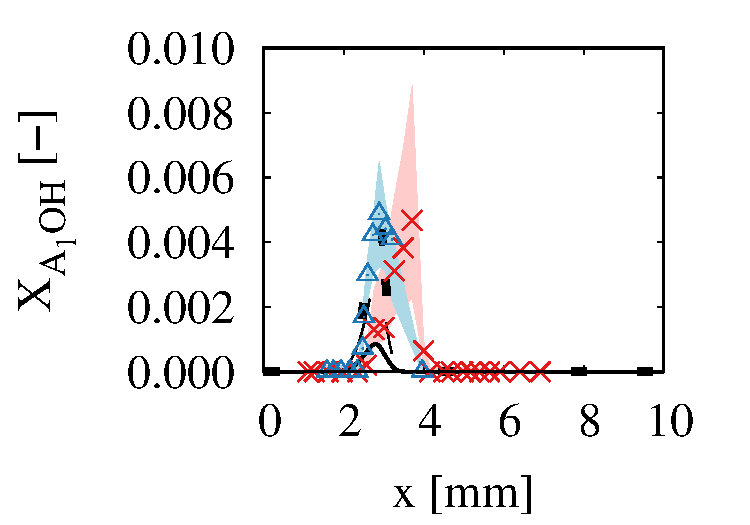
\includegraphics[width=0.32\textwidth]{\ThisPath Figures/B1b_Bio_Figure_12a.pdf}}
  \caption{Comparison of experimentally measured mole fractions in the \ce{CO2}F-Flame for anisole oxidation from Chen et al.~\cite{Chen2022} using the ToF-MBMS (red crosses), the GC-MS with a Rt-Q-Bond column (green circles), and the GC-MS with a DB-Petro column (blue triangles) with model predictions of the Skeletal-ITV-Bio (solid lines), the Merged-ITV-Anisole (dotted lines), and the LLNL-Anisole model~\cite{Wagnon2018} (dashed lines). Shaded areas with different colors indicate the measurement uncertainty of the respective techniques. x refers to the distance from the fuel inlet at 0 mm to the oxidizer inlet at 10 mm.}
  \label{fig:B1bAnisoleOxidationBioMechanism}
\end{figure}
\begin{figure}[h]
  \centering
  \subfloat{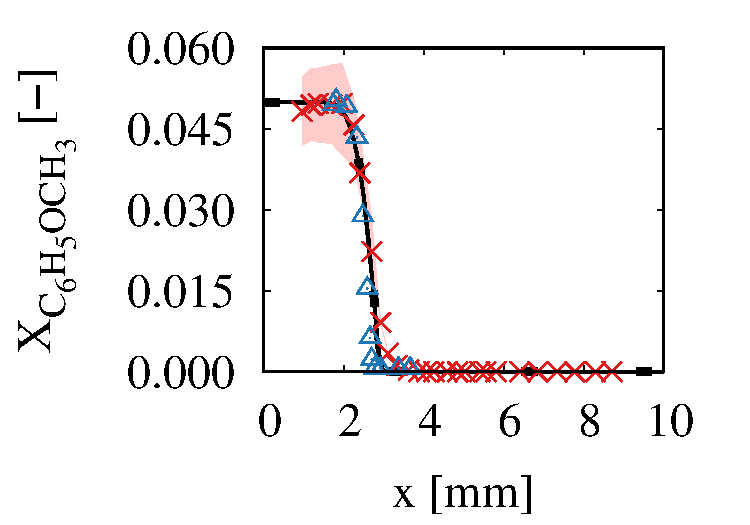
\includegraphics[width=0.32\textwidth]{\ThisPath Figures/B1b_Bio_Figure_6a.pdf}}
  \hfill
  \subfloat{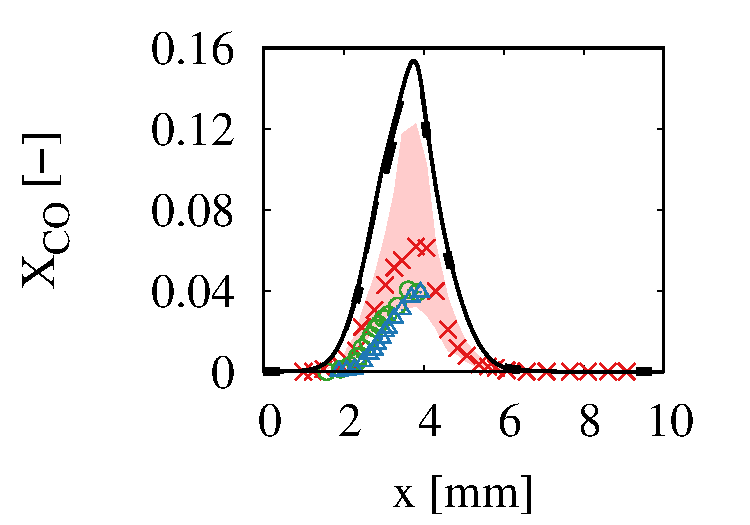
\includegraphics[width=0.32\textwidth]{\ThisPath Figures/B1b_Bio_Figure_6e.pdf}}
  \hfill
  \subfloat{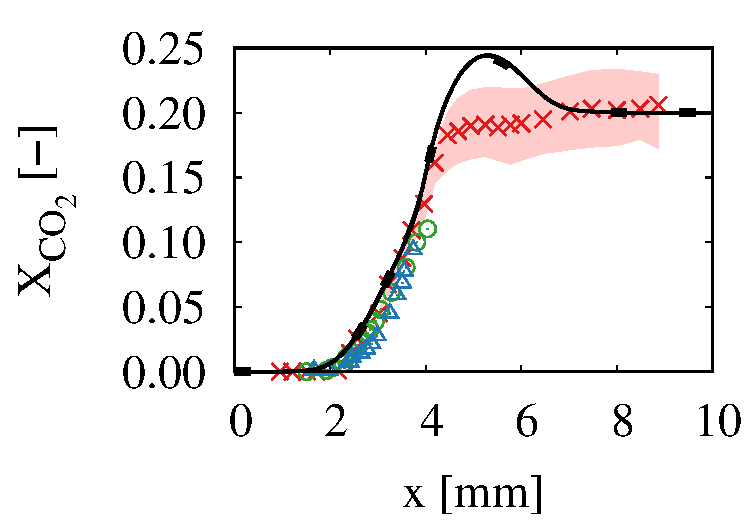
\includegraphics[width=0.32\textwidth]{\ThisPath Figures/B1b_Bio_Figure_6f.pdf}}
  \hfill
  \subfloat{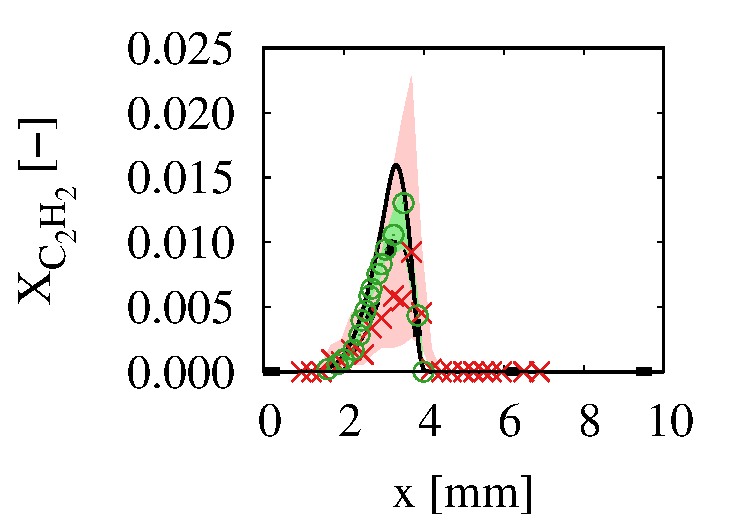
\includegraphics[width=0.32\textwidth]{\ThisPath Figures/B1b_Bio_Figure_8b.pdf}}
  \hfill
  \subfloat{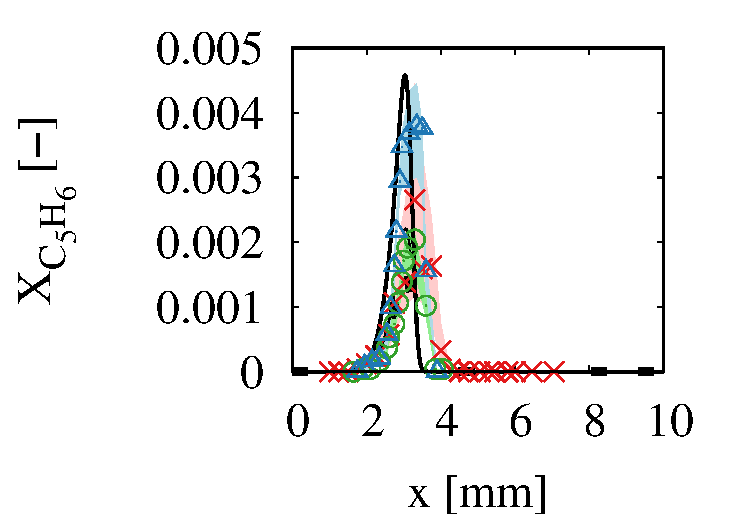
\includegraphics[width=0.32\textwidth]{\ThisPath Figures/B1b_Bio_Figure_8e.pdf}}
  \hfill
  \subfloat{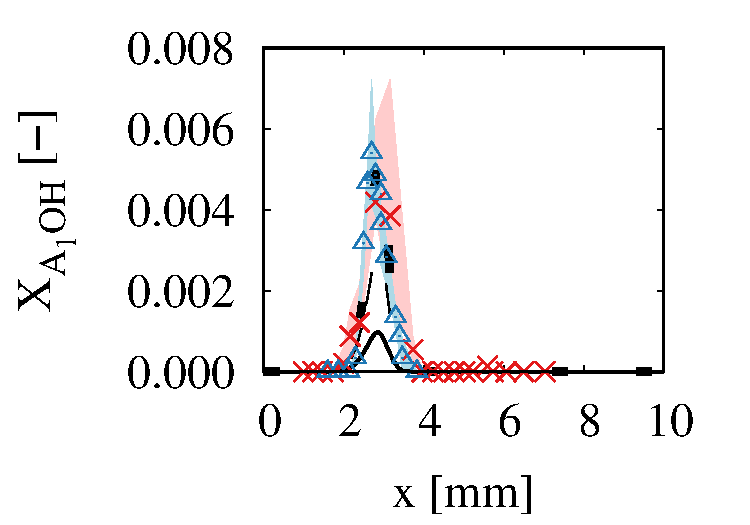
\includegraphics[width=0.32\textwidth]{\ThisPath Figures/B1b_Bio_Figure_13a.pdf}}
  \caption{Comparison of experimentally measured mole fractions in the \ce{CO2}O-Flame for anisole oxidation from Chen et al.~\cite{Chen2022} using the ToF-MBMS (red crosses), the GC-MS with a Rt-Q-Bond column (green circles), and the GC-MS with a DB-Petro column (blue triangles) with model predictions of the Skeletal-ITV-Bio (solid lines), the Merged-ITV-Anisole (dotted lines), and the LLNL-Anisole model~\cite{Wagnon2018} (dashed lines). Shaded areas with different colors indicate the measurement uncertainty of the respective techniques. x refers to the distance from the fuel inlet at 0 mm to the oxidizer inlet at 10 mm.}
  \label{fig:B1bAnisoleOxidationBioMechanismOXY}
\end{figure}



\subsection{Validation of the \ce{NOx} chemical kinetic sub-model}
\ce{NO_x}formation is validated for the volatile species released from the solid particle model in Cha.~\linkproject{A8} in a predefined range of validity for the Skeletal-ITV-\ce{NO_x} model. The Skeletal-ITV-\ce{NO_x} model is built on a reduced version of the well-documented Glarborg et al. model~\cite{Glarborg2022} with integrated ammonia chemistry from the KAUST model~\cite{Zhang2021}. Besides these applied validation cases, the newly developed Skeletal-ITV-\ce{NO_x} model will be validated for several N-containing species against experimental data under different conditions~\cite{Hulgaard199, Glarborg1994, Alzueta2002, Wu2019, Wu2022}.
\\
The Skeletal-ITV-\ce{NO_x} model is validated based on the model predictions of the Complete-ITV-\ce{NO_x} and the CRECK-\ce{NO_x} model~\cite{Shamooni2021} and to quartz flow reactor experiments for \ce{HCN} oxidation in Fig.~\ref{fig:B1bNOxBaseChemistry}. Both ITV-based kinetic models capture experimental measurements for \ce{CO2} and for the oxidation chemistry of \ce{HCN}, while the CRECK-\ce{NO_x} model~\cite{Shamooni2021} under-predicts the formation of both species. Minor prediction accuracy advantages of the kinetic models from the ITV are shown for \ce{HNCO} and \ce{N2O} in comparison to the CRECK-\ce{NO_x} model~\cite{Shamooni2021} in Fig.~\ref{fig:B1bNOxBaseChemistry}.
\begin{figure}[h]
  \centering
  \subfloat{\includegraphics[width=0.48\textwidth]{\ThisPath Figures/B1b_NOx_Glarborg2018_HCN_withoutCO_CPollutants.pdf}}
  \hfill
  \subfloat{\includegraphics[width=0.48\textwidth]{\ThisPath Figures/B1b_NOx_Glarborg2018_HCN_withoutCO_NPollutants.pdf}}
  \caption{Comparison of quartz flow reactor experimental data (symbols) from Hulgaard and Dam-Johansen~\cite{Hulgaard199} and Glarborg and Miller~\cite{Glarborg1994} in a quartz flow reactor for HCN oxidation and model predictions of the Skeletal ITV-\ce{NO_x} (solid lines), the Complete-ITV-\ce{NO_x} (dotted lines), and the CRECK-\ce{NO_x} model~\cite{Shamooni2021} (dashed lines).}
  \label{fig:B1bNOxBaseChemistry}
\end{figure}
\\
Figure~\ref{fig:B1bNOxWuValidation} compares the model predictions of the Skeletal-ITV-\ce{NO_x} with the model predictions of the Complete-ITV-\ce{NO_x} and the CRECK-\ce{NO_x} model~\cite{Shamooni2021} as well as with experimental measurements for different stoichiometry from Wu et al.~\cite{Wu2019, Wu2022}. The integrated \ce{C5H5N}-chemistry shows no discrepancies for both stoichiometries, while the \ce{NO} and \ce{NH3} model predictions from the ITV-based models are closer to the experimental measurements under both conditions than the CRECK-\ce{NO_x} model~\cite{Shamooni2021}. Model predictions of the Skeletal-ITV-\ce{NO_x} and the Compact-ITV-\ce{NO_x} model show no discrepancies, indicating that the neglected pathways in the reduction step have only a minor error on the target species.
%applied reduction step in the development introduces only a minor error on the pathways of the volatile species released from the solid \ce{NOx} sub-model from Cha.~\linkproject{A8}.
\begin{figure}[h]
  \centering
  \subfloat{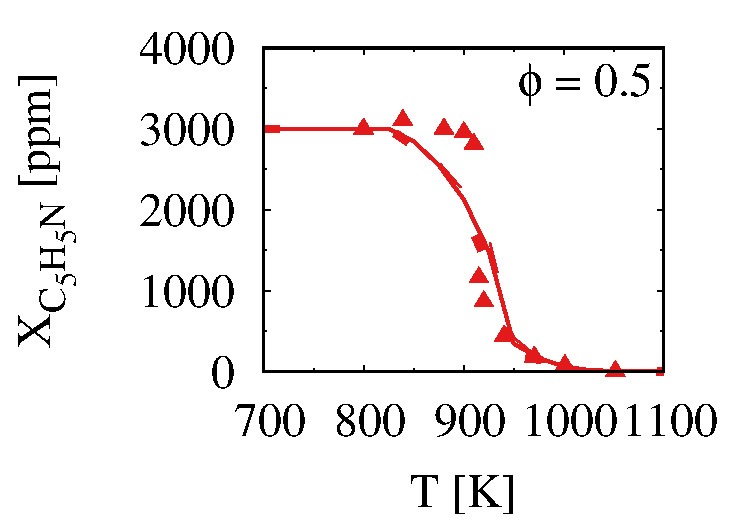
\includegraphics[width=0.32\textwidth]{\ThisPath Figures/B1b_NOx_Wu_Lean_C5H5N.pdf}}
  \hfill
  \subfloat{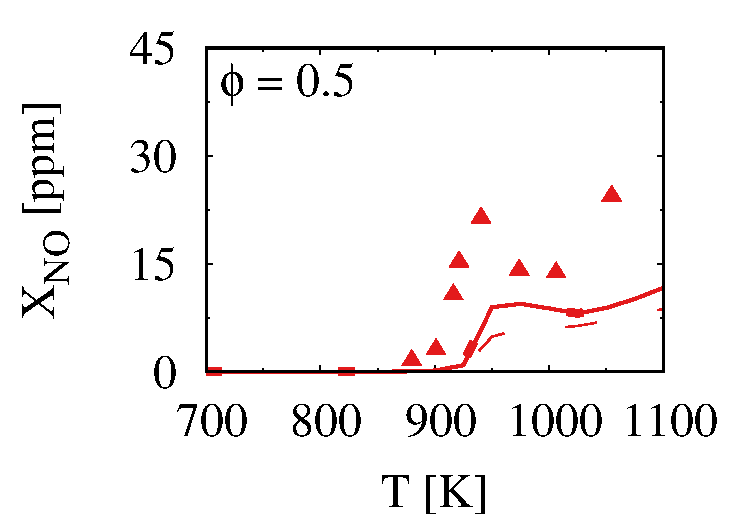
\includegraphics[width=0.32\textwidth]{\ThisPath Figures/B1b_NOx_Wu_Lean_NO.pdf}}
  \hfill
  \subfloat{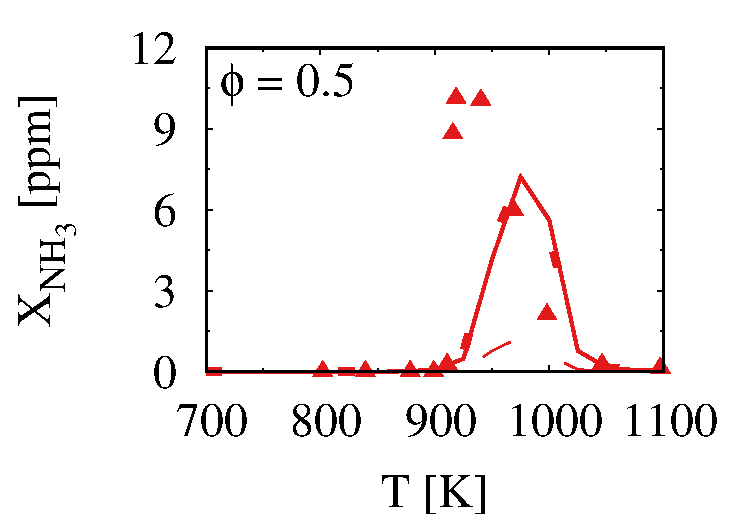
\includegraphics[width=0.32\textwidth]{\ThisPath Figures/B1b_NOx_Wu_Lean_NH3.pdf}}
  \hfill
  \subfloat{\includegraphics[width=0.32\textwidth]{\ThisPath Figures/B1b_NOx_Wu_Rich_C5H5N.pdf}}
  \hfill
  \subfloat{\includegraphics[width=0.32\textwidth]{\ThisPath Figures/B1b_NOx_Wu_Rich_NO.pdf}}
  \hfill
  \subfloat{\includegraphics[width=0.32\textwidth]{\ThisPath Figures/B1b_NOx_Wu_Rich_NH3.pdf}}
  \caption{Comparison of experimental data from Wu et al. ~\cite{Wu2019, Wu2022} in a jet-stirred reactor (symbols) and model predictions of the Skeletal ITV-\ce{NO_x} (solid lines), the Complete-ITV-\ce{NO_x} (dotted lines), and the CRECK-\ce{NO_x}  model~\cite{Shamooni2021} (dashed lines).}
  \label{fig:B1bNOxWuValidation}
\end{figure}




%%%% DON'T CHANGE ANYTHING FROM HERE UNTIL NEXT MARKER!
\Acknowledgement

%\ThisPath 
\renewcommand{\bibname}{References}
\printbibliography[heading=subbibliography]

\end{refsection}
%%%% DONT CHANGE ANYTHING UNTIL HERE!
